\section{Inside the Postconciliar Roman Sanctuary}
Walking into a Catholic church for Mass, a worshiper encounters stone, linen, metal, wax, parchment, and woven cloth arranged with centuries of liturgical memory. Forty principal furnishings, vessels, linens, books, service items, and vestments of the postconciliar Roman sanctuary are gathered in the plates that follow, showing what each object is, how the Church uses it in worship, what grounded symbolism the liturgy attaches to it, and how it continues or differs from the 1962 Roman Missal.

\PCDPlateHeader{Plate I --- The Postconciliar Roman Sanctuary}{Not to common scale (architectural perspective)}
\ifdefined\TriptychPrintEdition
\begin{center}
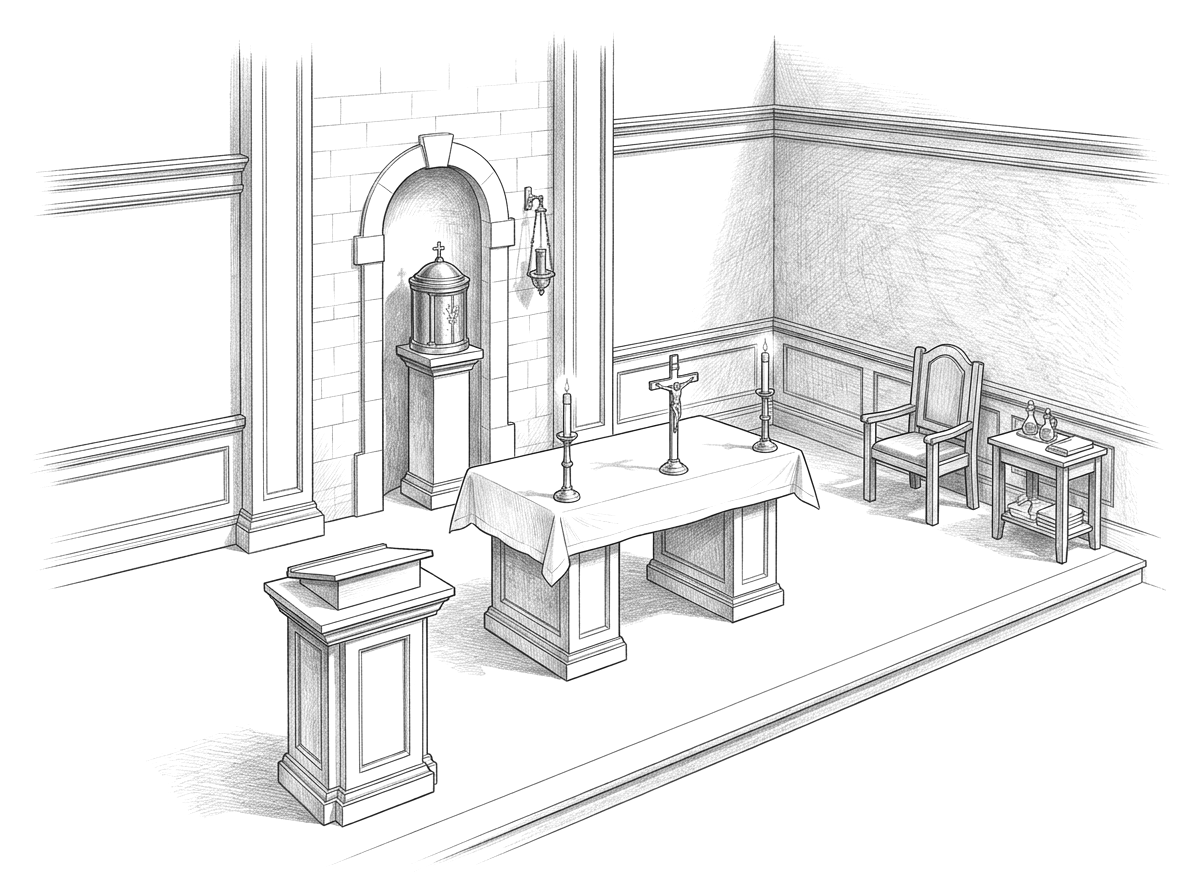
\includegraphics[width=0.96\linewidth,height=4.25in,keepaspectratio]{liturgy/roman-rite/postconciliar/2008-latin-2011-us-english/reference/roman-sanctuary-dictionary/shared/artwork/graphite/pc-art-01-sanctuary-composition.png}
\end{center}
\PCDPositionKey{Center: freestanding Altar with white Altar Cloth, two Altar Candles, and Altar Cross with corpus; foreground left: stationary Ambo; rear recessed niche: solid locked Tabernacle with hanging Sanctuary Lamp; rear right: Presidential Chair beside Credence Table holding cruets and linens.}
\else
\textbf{Visual Plate Summary (Plate I --- The Postconciliar Roman Sanctuary, Not to common scale (architectural perspective)):} Full architectural monochrome graphite perspective of a postconciliar Roman Catholic sanctuary showing the spatial coordination of freestanding stone altar dressed in white cloth with two candles and crucifix, permanent stone ambo in left foreground, wooden presidential chair and credence table with glass cruets and folded linens on the right, and a solid architectural tabernacle on a pillar inside a recessed arched niche with a hanging sanctuary lamp beside it. No altar cards, gradines, or rail appear.

\textbf{Reading order and object placement:} Center: freestanding Altar with white Altar Cloth, two Altar Candles, and Altar Cross with corpus; foreground left: stationary Ambo; rear recessed niche: solid locked Tabernacle with hanging Sanctuary Lamp; rear right: Presidential Chair beside Credence Table holding cruets and linens.
\fi

\subsection*{Monochrome Key for Liturgical Vestment Colors}
In monochrome graphite plates, vestment and textile colors appointed in the General Instruction of the Roman Missal (no.~346, with United States adaptations) are named in words and keyed below rather than encoded by tint alone.

\ifdefined\TriptychPrintEdition
{\footnotesize\begin{longtable}{>{\raggedright\arraybackslash}p{0.14\linewidth}>{\raggedright\arraybackslash}p{0.27\linewidth}>{\raggedright\arraybackslash}p{0.52\linewidth}}
\toprule
\textbf{Color} & \textbf{Monochrome key} & \textbf{Appointed occasions (US 2011 GIRM 346)} \\
\midrule
\endhead
\textbf{White} & \tikz[baseline=-0.5ex]{\draw[black,line width=0.5pt,fill=white] (0,0) rectangle (0.34cm,0.22cm);}\ Open white box (unshaded) & Easter Time, Christmas Time, celebrations of the Lord (except Passion), Blessed Virgin Mary, Angels, non-martyr Saints, All Saints, St. John the Baptist, St. John the Evangelist, Chair of St. Peter, Conversion of St. Paul; also permitted in the United States for funeral Masses (US GIRM 346e). \\
\textbf{Red} & \tikz[baseline=-0.5ex]{\draw[black,line width=0.5pt,pattern=vertical lines] (0,0) rectangle (0.34cm,0.22cm);}\ Vertical parallel rule & Palm Sunday of the Passion of the Lord, Good Friday, Pentecost Sunday, celebrations of the Passion of the Lord, birthdays (martyrdoms) of Apostles and Evangelists, and celebrations of Martyr Saints (GIRM 346b). \\
\textbf{Green} & \tikz[baseline=-0.5ex]{\draw[black,line width=0.5pt,pattern=north east lines] (0,0) rectangle (0.34cm,0.22cm);}\ Diagonal rising hatch & Offices and Masses of Ordinary Time (GIRM 346c). \\
\textbf{Violet} & \tikz[baseline=-0.5ex]{\draw[black,line width=0.5pt,pattern=crosshatch] (0,0) rectangle (0.34cm,0.22cm);}\ Cross-hatched grid & Advent and Lent; also lawful for Offices and Masses for the Dead (GIRM 346d). \\
\textbf{Black} & \tikz[baseline=-0.5ex]{\draw[black,line width=0.5pt,fill=black] (0,0) rectangle (0.34cm,0.22cm);}\ Solid black fill & Permitted where customary (including in the United States) for Masses for the Dead (US GIRM 346e). \\
\textbf{Rose} & \tikz[baseline=-0.5ex]{\draw[black,line width=0.5pt,pattern=dots] (0,0) rectangle (0.34cm,0.22cm);}\ Fine stippled dots & Permitted where customary on Gaudete Sunday (Third Sunday of Advent) and Laetare Sunday (Fourth Sunday of Lent) (GIRM 346f). \\
\textbf{Gold or Silver} & \tikz[baseline=-0.5ex]{\draw[black,line width=0.6pt] (0,0) rectangle (0.34cm,0.22cm); \draw[black,line width=0.3pt] (0.04cm,0.04cm) rectangle (0.30cm,0.18cm);}\ Double-bordered festive frame & Festive vestments may be worn on more solemn occasions even if not of the color of the day (GIRM 346g); in the United States, gold- or silver-colored vestments are permitted on more solemn occasions (US GIRM 346h). \\
\bottomrule
\end{longtable}}
\else
{\footnotesize\begin{longtable}{>{\raggedright\arraybackslash}p{0.14\linewidth}>{\raggedright\arraybackslash}p{0.25\linewidth}>{\raggedright\arraybackslash}p{0.54\linewidth}}
\toprule
\textbf{Color} & \textbf{Print pattern key} & \textbf{Appointed occasions (US 2011 GIRM 346)} \\
\midrule
\endhead
\textbf{White} & Open white box (unshaded) & Easter Time, Christmas Time, celebrations of the Lord (except Passion), Blessed Virgin Mary, Angels, non-martyr Saints, All Saints, St. John the Baptist, St. John the Evangelist, Chair of St. Peter, Conversion of St. Paul; also permitted in the United States for funeral Masses (US GIRM 346e). \\
\textbf{Red} & Vertical parallel rule & Palm Sunday of the Passion of the Lord, Good Friday, Pentecost Sunday, celebrations of the Passion of the Lord, birthdays (martyrdoms) of Apostles and Evangelists, and celebrations of Martyr Saints (GIRM 346b). \\
\textbf{Green} & Diagonal rising hatch & Offices and Masses of Ordinary Time (GIRM 346c). \\
\textbf{Violet} & Cross-hatched grid & Advent and Lent; also lawful for Offices and Masses for the Dead (GIRM 346d). \\
\textbf{Black} & Solid black fill & Permitted where customary (including in the United States) for Masses for the Dead (US GIRM 346e). \\
\textbf{Rose} & Fine stippled dots & Permitted where customary on Gaudete Sunday (Third Sunday of Advent) and Laetare Sunday (Fourth Sunday of Lent) (GIRM 346f). \\
\textbf{Gold or Silver} & Double-bordered festive frame & Festive vestments may be worn on more solemn occasions even if not of the color of the day (GIRM 346g); in the United States, gold- or silver-colored vestments are permitted on more solemn occasions (US GIRM 346h). \\
\bottomrule
\end{longtable}}
\fi

\clearpage
\PCDPlateHeader{Plate II --- Principal Sanctuary Furnishings}{Not to common scale}
\ifdefined\TriptychPrintEdition
\begin{center}
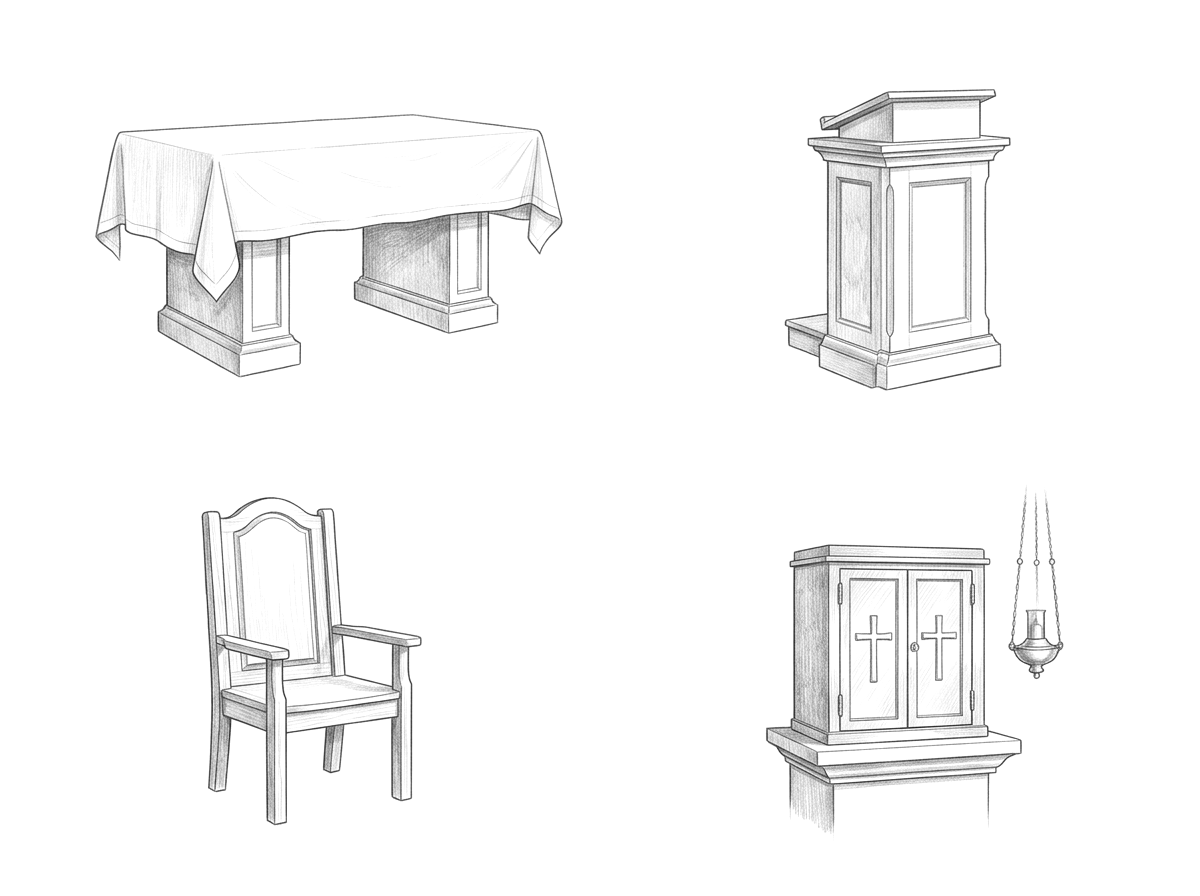
\includegraphics[width=0.92\linewidth,height=3.55in,keepaspectratio]{liturgy/roman-rite/postconciliar/2008-latin-2011-us-english/reference/roman-sanctuary-dictionary/shared/artwork/graphite/pc-art-02-altar-ambo-chair.png}
\end{center}
\PCDPositionKey{Top left: freestanding Altar covered with white linen cloth; top right: stationary stone Ambo with sloped desk and step; bottom left: dignified wooden Presidential Chair; bottom right: locked double-door Tabernacle on stone pedestal beside suspended oil Sanctuary Lamp.}
\else
\textbf{Visual Plate Summary (Plate II --- Principal Sanctuary Furnishings, Not to common scale):} Four-subject monochrome graphite architectural study comparing the principal sanctuary furnishings: top left, a freestanding carved stone altar dressed in a white linen altar cloth; top right, a permanent paneled stone ambo with angled book rest and rear step; bottom left, a stately wooden presidential chair with armrests; bottom right, a solid locked double-door metal tabernacle on a stone pedestal with a suspended sanctuary lamp burning beside it.

\textbf{Reading order and object placement:} Top left: freestanding Altar covered with white linen cloth; top right: stationary stone Ambo with sloped desk and step; bottom left: dignified wooden Presidential Chair; bottom right: locked double-door Tabernacle on stone pedestal beside suspended oil Sanctuary Lamp.
\fi

\label{pc-obj-altar}
\PCDEntryHead{Altar}{Altare}{required}{N01}
\PCDField{Also called}{Altar Table; Mensa; \textit{Mensa Domini}; \textit{Altare fixum}; \textit{Altare mobile}}
Standing at the focal center of the church, the altar is both the sacrificial table of Calvary made present in the Mass and the banquet table of the Lord's Body and Blood. Postconciliar churches ordinarily build one freestanding fixed altar---traditionally of natural stone, or in the United States also of dignified solid wood---so the priest can move around it and face the gathered assembly where architecture allows. Stripped of clutter before the offertory and clothed in crisp white linen, the altar directs every eye to the Eucharistic offering.

\PCDField{On the plate}{Top left (Plate II); center (Plate I)}
\PCDField{Symbolism}{The Church reveres the altar as the sign of Christ Himself---both Priest and Victim---and as the table of the Lord where the Sacrifice of the Cross is made present under sacramental signs. A fixed stone altar permanently signifies Christ the Living Stone, recalling 1 Pet 2:4 (``Unto whom coming, as to a living stone, rejected indeed by men but chosen and made honourable by God:''), 1 Cor 10:4 (``and the rock was Christ.''), and Heb 13:10 (``We have an altar whereof they have no power to eat who serve the tabernacle.''). St. Thomas Aquinas similarly teaches that the altar signifies Christ Himself and, when made of stone, calls to mind both Christ the Rock and the stone sepulchre in which His body rested. (GIRM 296, 298; 1 Pet 2:4; 1 Cor 10:4; Heb 13:10; St. Thomas Aquinas, Summa Theologiae III, q. 83, a. 3)}
\PCDField{Relation to the 1962 Missal}{\PCDTag{materially changed} Whereas the 1962 Roman Missal ordinarily presupposed a stone altar (or recessed consecrated altar stone holding relics inside the mensa) dressed with three cloths, candlesticks, central crucifix, three altar cards, and normally the tabernacle, the 2008/2011 Missal recommends a single freestanding altar wherever possible (GIRM 299, 303), deposits saints' relics beneath the altar (GIRM 302), clears the mensa of altar cards and extraneous items (GIRM 306), and in the United States permits solid wood for a fixed altar mensa (US GIRM 301).}
\PCDEntryRule

\label{pc-obj-ambo}
\PCDEntryHead{Ambo}{Ambo}{required}{N02}
\PCDField{Also called}{Lectern of the Word; \textit{Lectrinum}}
Because Catholic worship nourishes the faithful at two tables---the table of God's Word and the table of Christ's Body---the postconciliar sanctuary pairs its central altar with a solid, stationary ambo. Built to match the altar's dignity rather than serving as a utilitarian podium, the ambo is set apart strictly for Scripture, the Responsorial Psalm, the Easter Proclamation, the homily, and the Prayer of the Faithful, drawing the entire assembly's gaze when God speaks through the sacred readings.

\PCDField{On the plate}{Top right (Plate II); left foreground (Plate I)}
\PCDField{Symbolism}{The General Instruction pairs the ambo with the altar as the two tables of the Mass---the table of God's Word and the table of Christ's Body---directing that the dignity of Sacred Scripture be honored by a fixed, noble place toward which the congregation naturally turns. Its prominence visibly echoes the Psalmist's confession in Ps 118:105 [Heb 119:105]: ``Thy word is a lamp to my feet, and a light to my paths.'' (GIRM 28, 309; Ordo lectionum Missae (1981) Praenotanda 32--34; Ps 118:105 [Heb 119:105])}
\PCDField{Relation to the 1962 Missal}{\PCDTag{newly provided} The 1962 Roman Missal did not prescribe a permanent sanctuary ambo: at Low Mass the priest read the Epistle and Gospel from opposite corners of the altar, and at Solemn Mass the subdeacon and deacon sang them from the sanctuary floor with the subdeacon holding the Gospel book (RS VI.4--5). Postconciliar law restores a dedicated stationary ambo as a standard architectural appointment of every sanctuary (Inter Oecumenici 96; GIRM 309).}
\PCDEntryRule

\label{pc-obj-presidential-chair}
\PCDEntryHead{Presidential Chair}{Sedes sacerdotis celebrantis}{required}{N03}
\PCDField{Also called}{Chair for the Priest Celebrant; Presider's Chair; \textit{Sedes}}
In the postconciliar Roman sanctuary, the priest celebrant presides over the opening prayers, the Liturgy of the Word, and the final blessing from a distinct single chair before moving to the altar for the Liturgy of the Eucharist. Its noble simplicity expresses the priest's spiritual office of leading the assembly in prayer as head of the local gathering, while deliberately avoiding the canopy or trappings of a royal throne.

\PCDField{On the plate}{Bottom left (Plate II); rear right (Plate I)}
\PCDField{Symbolism}{The General Instruction assigns the presidential chair a clear functional sign value: it manifests the priest celebrant's office of presiding over the gathered assembly and directing its prayer, while explicitly excluding any likeness to a royal throne. (GIRM 310)}
\PCDField{Relation to the 1962 Missal}{\PCDTag{materially changed} In the 1962 Roman Rite, presbyteral seating consisted of a three-seat bench (sedilia) placed along the Epistle side of the sanctuary solely for sitting during sung chants and lessons while all orations were spoken at the altar. Postconciliar law replaces those lateral seats with a focal single chair from which the priest leads the Introductory Rites, Liturgy of the Word, and Concluding Rites (Inter Oecumenici 92; GIRM 310).}
\PCDEntryRule

\label{pc-obj-credence-table}
\PCDEntryHead{Credence Table}{Abacus}{required}{N04}
\PCDField{Also called}{Side Table; Credence; \textit{Credentia}; \textit{Mensa credentiae}}
Tucked unobtrusively to one side of the sanctuary, the credence table performs an essential practical service: it holds the chalice, paten, cruets, handwashing basin, and altar linens before they are brought to the altar at the offertory. By staging every necessary article within quiet reach of the servers and clergy, it allows the main altar table to remain visually calm and uncluttered until the Liturgy of the Eucharist begins.

\PCDField{On the plate}{See Plate I, far right beside the presidential chair}
\PCDField{Relation to the 1962 Missal}{\PCDTag{continued} Both the 1962 Roman Missal (RG 528; RS II.5) and the 2008/2011 GIRM (118c, 139, 279) appoint a sanctuary side table (abacus) for cruets, lavabo articles, Communion-plate, and vessels. In postconciliar Mass with a congregation, its role expands because the chalice and linens also ordinarily wait there until the Preparation of the Gifts (rather than being carried to the altar by the priest at the start of Low Mass) and vessel purification commonly takes place at the credence table (GIRM 279).}
\PCDEntryRule

\label{pc-obj-tabernacle}
\PCDEntryHead{Tabernacle}{Tabernaculum}{required}{N05}
\PCDField{Also called}{Eucharistic Tabernacle}
Set in a prominent, quiet place of honor, the tabernacle is the locked sacred dwelling where consecrated hosts are kept after Mass so that Christ can be carried immediately to the sick and dying as Viaticum and adored by the faithful in silent prayer. Postconciliar Roman law places the tabernacle apart from the altar of celebration---either elsewhere in the sanctuary or in an adjoining Blessed Sacrament chapel as the Diocesan Bishop decides---so that worshipers clearly distinguish the unfolding Eucharistic action at the altar from Christ's abiding presence in reservation.

\PCDField{On the plate}{Bottom right (Plate II); recessed rear niche (Plate I)}
\PCDField{Symbolism}{The Church honors the tabernacle as the consecrated dwelling of Christ's abiding sacramental presence in the midst of His people, recalling the Lord's promise to Israel in Ex 25:8 (``And they shall make me a sanctuary, and I will dwell in the midst of them:''). Setting the tabernacle apart from the altar of celebration keeps distinct the sign of Christ's reserved presence for adoration and Viaticum from the sacrificial action of Mass, fulfilling the constant pastoral care that St. Thomas Aquinas grounds in bringing the Eucharist to the sick without delay. (GIRM 314--315; Eucharisticum Mysterium (1967) 53--55; Ex 25:8; St. Thomas Aquinas, Summa Theologiae III, q. 83, a. 5, ad 11)}
\PCDField{Relation to the 1962 Missal}{\PCDTag{materially changed} Both the 1917 Code (cann. 1268--1269) and current law (CIC 1983 can. 938; GIRM 314) mandate a single immovable, solid, opaque, securely locked tabernacle. Whereas 1917/1962 discipline ordinarily fixed the veiled tabernacle in the middle of the high altar of celebration, GIRM 315 considers it clearer as a sign not to place it on the altar where Mass is celebrated, entrusting the Diocesan Bishop to choose either another worthy place in the sanctuary or an organically connected adoration chapel, and no longer universally mandating a tabernacle veil.}
\PCDEntryRule

\label{pc-obj-sanctuary-lamp}
\PCDEntryHead{Sanctuary Lamp}{Lampas peculiaris}{required}{N06}
\PCDField{Also called}{Tabernacle Lamp; Presence Lamp; \textit{Lampas sanctuarii}; \textit{Lucerna}}
Hanging quietly beside the tabernacle, the sanctuary lamp is the Church's silent beacon announcing that Christ is sacramentally present inside. Fed continuously by real oil or wax in fidelity to ancient biblical and Roman custom, its single steadfast flame invites every worshiper entering the church to pause, genuflect, and pray before the Lord.

\PCDField{On the plate}{Suspended beside the tabernacle at bottom right (Plate II) and in the rear niche (Plate I)}
\PCDField{Symbolism}{The continuously burning oil or wax lamp openly signals Christ's abiding sacramental presence in the tabernacle and renders silent honor to Him day and night, echoing the perpetual lamp commanded before the Old Covenant sanctuary in Ex 27:20--21 (``Command the children of Israel that they bring thee the purest oil of the olives, and beaten with a pestle: that a lamp may burn always, In the tabernacle of the testimony, without the veil that hangs before the testimony'') and Lev 24:2--3 (``to furnish the lamps continually, Without the veil of the testimony in the tabernacle of the covenant''). (GIRM 316; CIC (1983) can. 940; Ex 27:20--21; Lev 24:2--3)}
\PCDField{Relation to the 1962 Missal}{\PCDTag{continued} Postconciliar discipline continues the 1917/1962 requirement without interruption: both CIC (1917) can. 1271 and CIC (1983) can. 940 together with GIRM 316 require a special living flame of oil or wax to burn continually before or near the tabernacle whenever the Eucharist is reserved.}
\PCDEntryRule

\label{pc-obj-baptismal-font}
\PCDEntryHead{Baptismal Font}{Fons baptismalis}{required}{N07}
\PCDField{Also called}{Font; \textit{Fons baptismatis}}
Required in every parish church by canon law, the baptismal font marks the threshold of Christian life where believers are reborn of water and the Holy Spirit. Traditionally carved with eight sides to recall the eighth day of Christ's Resurrection, the postconciliar font is placed prominently where the whole parish can gather around it for Baptisms and return to it during the Easter Vigil to renew their baptismal promises.

\PCDField{On the plate}{See Plate X, bottom right}
\PCDField{Symbolism}{The ancient Roman Easter Vigil blessing calls the baptismal font the motherly womb from which the Church brings forth new children in Christ, uniting the Lord's teaching in John 3:5 (``unless a man be born again of water and the Holy Ghost, he cannot enter into the kingdom of God.'') with St. Paul's mystery of death and resurrection in Rom 6:3--4 (``Know you not that all we who are baptized in Christ Jesus are baptized in his death? For we are buried together with him by baptism into death: that, as Christ is risen from the dead by the glory of the Father, so we also may walk in newness of life.''). Early Christian catechesis, including St. Cyril of Jerusalem, expounds the font as both tomb and womb of new creation, reflected architecturally in the classic octagonal basin of the eighth day. (Roman Missal Easter Vigil; CCC 1237--1243; John 3:5; Rom 6:3--4; St. Cyril of Jerusalem, Mystagogical Catechesis 2.4)}
\PCDField{Relation to the 1962 Missal}{\PCDTag{materially changed} Both 1962 discipline and CIC (1983) can. 858 require a baptismal font in every parish church. Whereas 1962 practice ordinarily enclosed the font inside a gated baptistery near the church entrance and blessed the year's water at the Easter Vigil with an infusion of Oil of Catechumens and Sacred Chrism directly into the basin, postconciliar rites bless fresh water at each Baptism outside Easter Time without pouring oils into the font and favor congregationally visible placement suited to pouring or immersion.}
\PCDEntryRule
